\chapter{Design}
\thispagestyle{main} % Needed for Footer and Header on Chapterpage
This chapter outlines the design of the Bazo Virtual Machine and all other components on given requirements and restrictions based on the previous work this project is based on. The following sections also describe how smart contracts are written, deployed and called in Solidity and in Bazo byte code instructions and what changes had to be made to the miner. Furthermore trade-offs regarding different virtual machine implementations are discussed. Figure \ref{vmexecutioncycle} shows all components of the virtual machine in one single diagram. All components and entities are described in detail in the following sections. Not shown in the diagram is the parser which is also documented in this section.

\begin{figure}[H]
	\begin{center}
	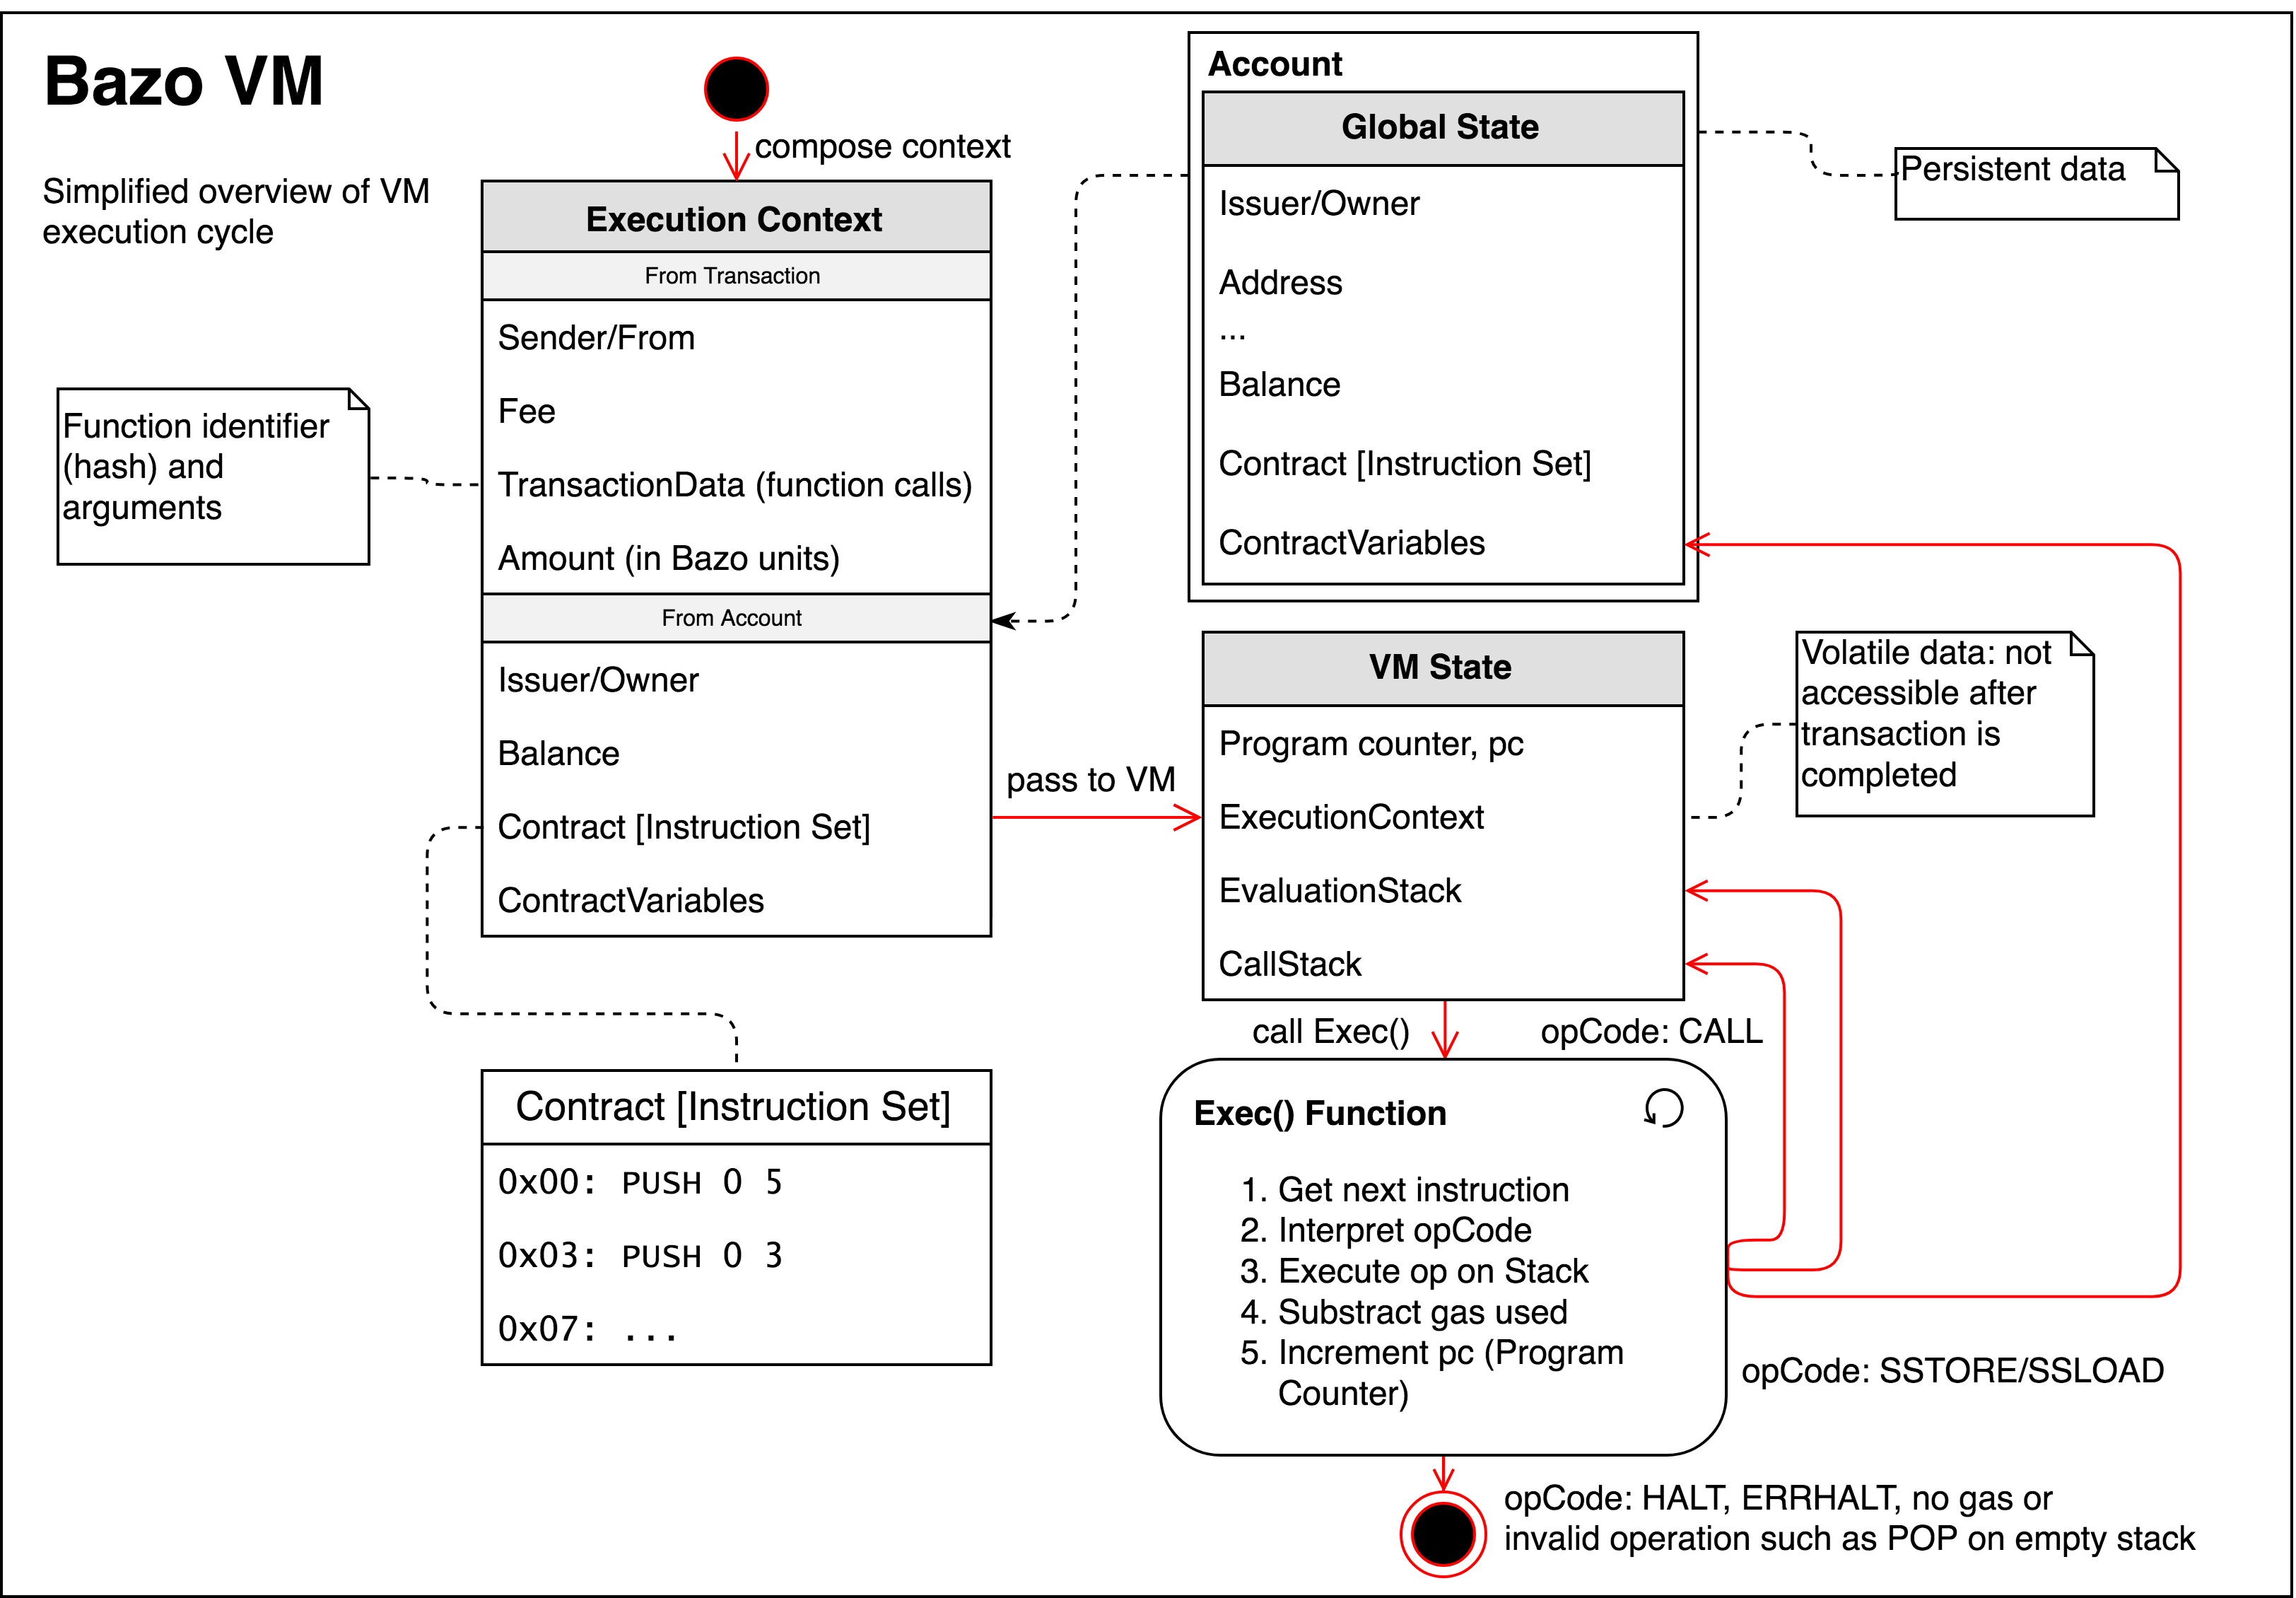
\includegraphics[width=\textwidth]{./images/execution-cycle}
	\caption{Virtual machine execution cycle}
	\label{vmexecutioncycle}
	\end{center}
\end{figure}

\section{From contract creation to the effects of execution}
\subsection{Contract deployment}
A user creates a contract via the command line interface client. There he provides the necessary parameters which include the code of the contract and the initial state variables and sends the transaction to the miner. The miner then validates the incoming transaction and creates an account according to the provided parameter on his heap memory, see section \ref{accounts} for further information about accounts. It also broadcasts the new transaction to the other miners, which then act accordingly.

\subsection{Execution of a contract method}
A user again creates a new transaction, see chapter to call a contract. He provides the necessary parameters and the hash of the function he wants to call in field of the new transaction. This new transaction again is transmitted to the miner, as he sees the type of the transaction that the data field is not empty it will find the called contract and execute its code according to the provided parameters in the data field. Now the user can check the updated state on the blockchain. 
\pagebreak

\section{Miner} \label{design_miner}
As mentioned before, the miner is responsible for processing and validating transactions. This sections describes the requirements and restrictions the integration of the virtual machine is based on. Furthermore, the changes that have to be made to the miner are documented.

\subsection{Transaction Types} \label{transactionTypes}
The miner comes with different types of transactions. 

\begin{tabular}[t]{ p{3cm} p{12.5cm}}
\raggedright
\textbf{FundsTx} &
This type of transaction is used to transfer Bazo coins from one account to another.\cite{ba_miner} The Data field was added, since the FundsTx is the ideal type of transaction to call smart contract functions.
\\ \\
\end{tabular}

\begin{figure}[thp]%
    	\centering
		\begin{minipage}{0.4\textwidth}
		\begin{minted}
		[
		frame=lines,
		autogobble,
		framesep=2mm,
		baselinestretch=1.2,
		fontsize=\footnotesize,
		linenos
		]
		{go}
		type FundsTx struct {
			Header byte
			Amount uint64
			Fee    uint64
			TxCnt  uint32
			From   [32]byte
			To     [32]byte
			Sig1   [64]byte
			Sig2   [64]byte
			Data   []byte
		}
		\end{minted}
		\end{minipage}
\end{figure}

\begin{tabular}[t]{ p{3cm} p{12.5cm}}
\raggedright
\textbf{AccTx} &
The AccTx is used to create a new account. As for now this type of transaction is only allowed to root accounts, since the signature has to be signed with the private key of a root account. \cite{ba_miner} Nevertheless this transaction type is the perfect foundation to create smart contract accounts. Therefore a contract field and a contract variable field were added. \\ \\
\end{tabular}

\begin{figure}[thp]%
    	\centering
		\begin{minipage}{0.4\textwidth}
		\begin{minted}
		[
		frame=lines,
		autogobble,
		framesep=2mm,		
		baselinestretch=1.2,
		fontsize=\footnotesize,
		linenos
		]
		{go}
		type AccTx struct {
			Header            byte
			Issuer            [32]byte
			Fee               uint64
			PubKey            [64]byte
			Sig               [64]byte
			Contract          []byte
			ContractVariables []big.Int
		}
		\end{minted}
		\end{minipage}
\end{figure}

\begin{tabular}[t]{ p{3cm} p{12.5cm}}
\raggedright
\textbf{ConfigTx} &
This type of transaction is used to change system parameters such as block size, block interval or minimum fee. \cite{ba_miner} This type of transaction is not discussed any further. \\ \\
\textbf{StakeTx} &
Since the Bazo Blockchain is in transition from proof of work to proof of stake consensus mechanism there is a StakeTx transaction type. This type of transaction is also not discussed any further.
\end{tabular}

\subsection{Accounts} \label{accounts}
Accounts are the result of processing an account transaction. They are object on the heap of the miner. The Bazo miner already had the transaction type to create accounts by design. There is only one struct for the the two different types of account. This is the struct for account:

\begin{figure}[thp]%
    	\centering
		\begin{minipage}{0.6\textwidth}
		\begin{minted}
		[
		frame=lines,
		autogobble,
		framesep=2mm,		baselinestretch=1.2,
		fontsize=\footnotesize,
		linenos
		]
		{go}
		type Account struct {
			Address            [64]byte  // 64 Byte
			Issuer             [32]byte  // 32 Byte
			Balance            uint64    // 8 Byte
			TxCnt              uint32    // 4 Byte
			IsStaking          bool      // 1 Byte
			HashedSeed         [32]byte  // 32 Byte
			StakingBlockHeight uint32    // 4 Byte
			Contract           []byte
			ContractVariables  []big.Int 
		}
		\end{minted}
		\end{minipage}
\end{figure}

\begin{tabular}[t]{ p{3cm} p{12.5cm}}
\raggedright
\textbf{Externally owned accounts} &
Externally owned accounts are accounts that are owned by the person who has access to the combination of the public and private key. Having both, the person is able to execute transaction from that account. The creation of externally owned accounts was already given by the previous thesis by Livio Sgier. A externally owned account does not have an Issuer, Contract and ContractVariables. \\ \\
\textbf{Smart contract accounts} &
Smart contracts accounts are created and owned by externally owned accounts. Smart contracts accounts have two additional fields, which were added to the account creation transaction. The issuer shows which externally owned account issued the contract account. A contract account has both, Contract and ContractVariables, fields set.

	\begin{description}
  		\item[Contract] This field contains the smart contract. The data type is byte slice, since a contract can have a variable length and contracts get compiled to byte code.
  		\item[ContractVariables] This field contains the state variables that can be altered by contract functions. The data type is a slice of big.Int since a contract can have a variable amount of variables.
	\end{description}
\end{tabular}

\section{Virtual Machine}
There are two types of virtual machines. On the one hand there are register based virtual machines. Examples of register based virtual machines are the Lua VM and the Dalvik VM. On the other there are stack based virtual machines. The Java Virtual Machine and the .NET CLR are both stack based virtual machines. \cite{stackvsregistervm}

\subsection{Register based}
The data structure of where the operands are stored is based on registers of the CPU, therefore the instructions need to contain the addresses (registers) of the operands. This leads to longer instructions. Figure \ref{register vm} shows how adding two number works on a register based virtual machine. \cite{stackvsregistervm} The instruction is \mintinline{tasm}{ADD R1 R3 R2}.

\begin{figure}[H]
	\begin{center}
	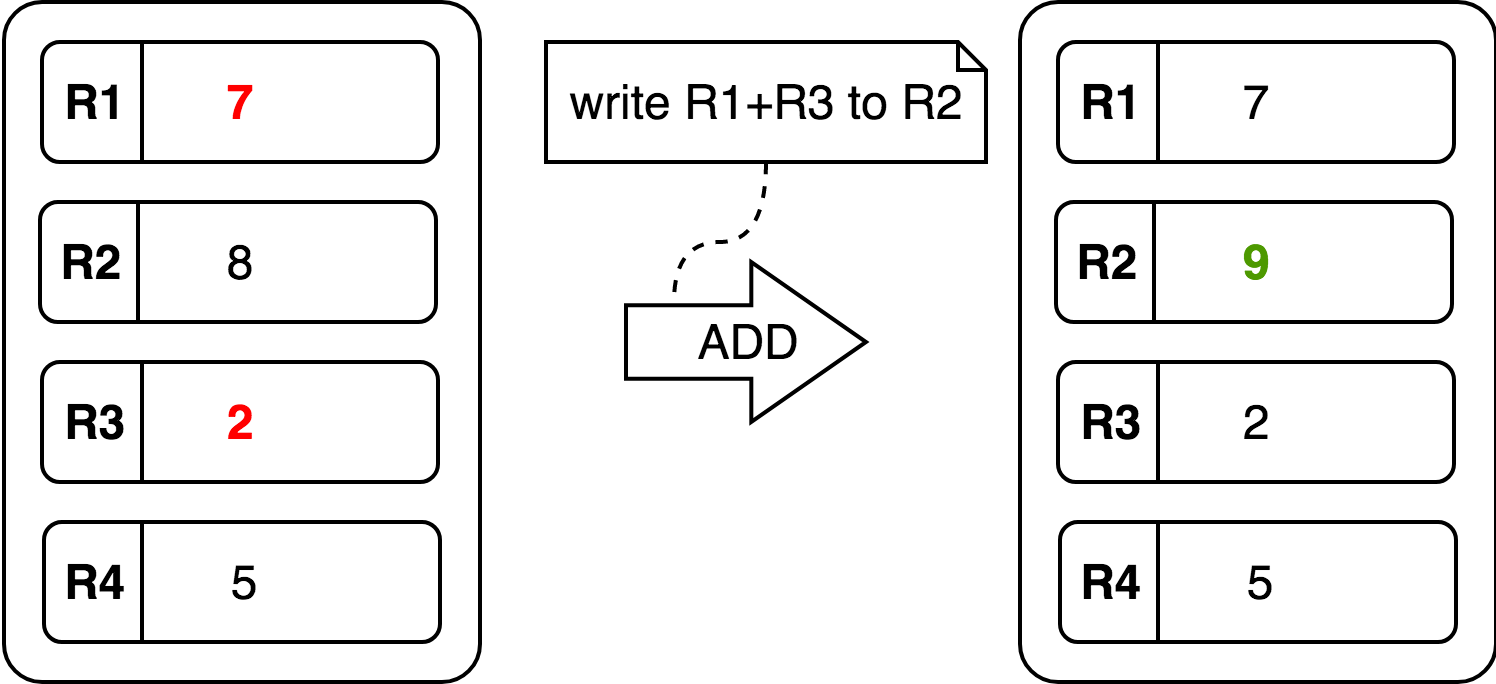
\includegraphics[width=0.61\textwidth]{./images/register-example}
	\caption{Register based virtual machine}
	\label{register vm}
	\end{center}
\end{figure}
  
\subsection{Stack based}
A stack based virtual machine is based on a LIFO (last in, first out) stack. Operations are carried out by popping and pushing back results on the stack. The main advantage is a stack pointer that implicitly addresses the operands, which means that no addresses are passed in instructions. The instructions code is longer since \mintinline{tasm}{POP} and \mintinline{tasm}{PUSH} instructions have to be included to retrieve and store the operands. \cite{stackvsregistervm} The instruction to add two numbers as shown in figure \ref{stack vm} are: 
  \begin{figure}[thp]%
    \centering
	\begin{minipage}{0.4\textwidth}
  \begin{minted}	[
	frame=lines,
	framesep=2mm,
	baselinestretch=1.2,
	fontsize=\footnotesize,
	linenos
	]
	{tasm}
	POP
	POP
	ADD
	PUSH
  \end{minted}
  \end{minipage}
  \end{figure}
  \begin{figure}[H]
	\begin{center}
	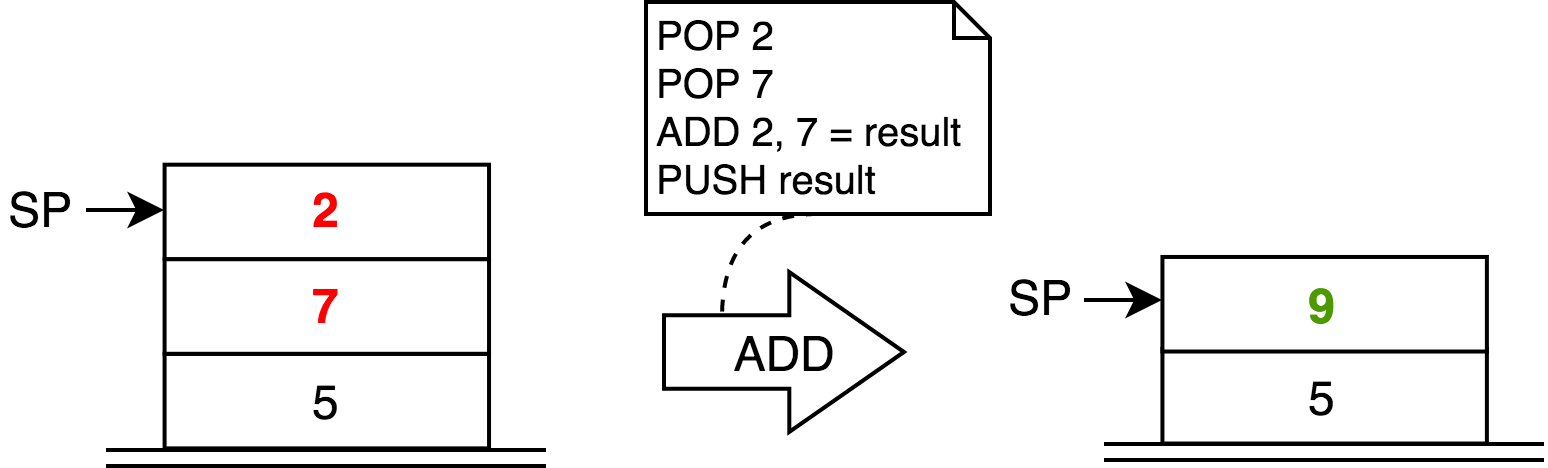
\includegraphics[width=0.6\textwidth]{./images/stack-example}
	\caption{Stack based virtual machine}
	\label{stack vm}
	\end{center}
  \end{figure}

\subsection{Design decision}
Despite the register based virtual machine having advantages such as more possibilities for optimizations and having no overhead from pushing and popping, over a stack based virtual machine we decided to implement a stack based virtual machine. This decision was most influenced by the implementation of related projects, namely Ethereum and NEO. Besides that, the implementation of a stack based virtual machine is simpler and much more resources are available. 

\subsection{VM Execution cycle} \label{exec_cycle}
This section describes the \mintinline{go}{Exec()} function shown in figure \ref{vmexecutioncycle}. The execution cycle can be described as an end-less loop with a switch statement that interprets the instructions one after another and acts accordingly.

\begin{tabular}[t]{ p{3cm} p{12.5cm}}
\raggedright
\textbf{Precondition} & 
The virtual machine is embedded into the miner. Precondition that the VM execution cycle is started is, that the transaction must be sent to a smart contract account and the transaction data field is not empty. If these preconditions can be fulfilled, the vm execution cycle is started by the miner. \\ \\

\textbf{Starting point} & 
The starting point for the execution cycle of the virtual machine is a set of instructions, an execution context, which are local state variables and an incrementing counter, called the program counter, which points to the instruction that is executed next. \\ \\

\textbf{Steps} &
The instruction cycle can be divided into three steps which are repeated over and over again until an invalid instruction occurs, the execution is halted by an instruction or the program counter is out of bounds of the instruction set. All this steps are handled in the \mintinline{go}{Exec()} function. This are the three steps:
\begin{description}
  \item[1. Fetch] The instruction of the instruction code where the program counter points to is fetched. After it is fetched, the program counter is increased.
    \end{description}
\end{tabular}

\begin{tabular}[t]{ p{3cm} p{12.5cm}}
\raggedright
\textbf{ } & 
\begin{description}
	\item[2. Decode] The instruction is interpreted by the decoder. The decoder matches the instructions with pre-defined opcodes, which can be interpreted by the execute function. Within this section of the function, the costs for the instruction are deducted. Section \ref{fee} describes why a fee is needed and how it is calculated.
    \item[3. Execute] The instruction is executed on the stack according to the opcode. There are opcodes for arithmetic operations, e.g. \mintinline{yaml}{ADD, MOD, SUB}, for flow operations e.g. \mintinline{yaml}{JMP, CALL, RET} which are allowed to change the program counter and therefore move back and forward in the instruction set, cryptographic operations, such as \mintinline{yaml}{SHA3, CHECKSIG} and context operations, e.g. \mintinline{yaml}{ADDRESS, ISSUER, CALLER, CALLDATA} that can be used to push context data composed from the transaction and the receiver account to the stack and opcodes for storing and loading state variables \mintinline{yaml}{SSTORE, SLOAD}. All implemented opcodes are listed in table \ref{opcodes cheat sheet}.
\end{description}
\end{tabular}

\begin{tabular}[t]{ p{3cm} p{12.5cm}}
\raggedright
\textbf{Return Value} &
The \mintinline{go}{Exec()} function returns a boolean. If the return value is true the execution was successful and no error or exception occurred. If the return value is false an error or exception occurred. \\ \\

\textbf{Persisting state variables} &
Changes to the state variables are loaded and persisted explicit. That means, when loading a state variable a copy is pushed to the stack, all changes are made to the copy. The changes are only persisted if the \mintinline{go}{Exec()} function returns with true, this way there is no need to roll back if the contract could not be executed successfully.
\end{tabular}

\section{Parser}
Since writing all contracts directly in byte code can be very complicated and time-consuming, we decided to write a very basic parser. The goal of the parser was to make writing contracts easier by allowing the usage of labels and comments. Having labels resolves the problem of counting addresses when using flow operation opcodes like \mintinline{yaml}{JMP} and \mintinline{yaml}{CALL} since they generally take an address as argument and change the program counter accordingly. Labels could also be interpreted as jump markers. The parser could also be used as foundation for building a compiler which translates a contract written in a high-level language into Bazo byte code. For the rest of this thesis the code that can be interpreted by the parser is referred to as \flqq Enhanced Bazo Byte Code\frqq{} and the code the virtual machine operates on and which is stored on the blockchain as \flqq Bazo Byte Code\frqq.

\subsection{\flqq Enhanced Bazo Byte Code\frqq{}}
Listing \ref{basiccontract_design} shows an example of a contract written in \flqq Enhanced Bazo Byte Code\frqq{}. It is possible to have single line comments and inline comments as well, as seen in line 1 and line 5. Comments and empty lines are ignored by the parser. The first word in line is either an opcodes or a label, which ends with a colon. Opcodes are optionally followed by arguments. It is predefined what type of arguments an opcode has. The \mintinline{go}{CALL} opcode in line 4 for instance takes a label and a byte as argument.

\begin{figure}[thp]%
    \centering
	\begin{minipage}{0.6\textwidth}
\begin{minted}
[
	frame=lines,
	framesep=2mm,
	baselinestretch=1.2,
	fontsize=\footnotesize,
	linenos
]
{yaml}
# This is a simple program which calls a function
PUSH 55780
PUSH 5
CALL addNums 2
HALT # stops execution

addNums:
LOAD 0
LOAD 1
ADD
RET
\end{minted}
\end{minipage}
\caption{Basic contract with function call written in \flqq Enhanced Bazo Byte Code\frqq{}}
\label{basiccontract_design}
\end{figure}

\subsection{Compile process}
First the parser splits the contract written in \flqq Enhanced Bazo Byte Code\frqq{}, which is basically only a long string, into tokens. A token consists of a token type and a value. The token type represents a kind of lexical unit e.g. opcode, label or a sequence of input characters. The token types are the symbols that are processed by the parser. \cite{aho_compilers:_2007} To get to the \flqq Bazo Byte Code\frqq{} the resulting set is iterated and the token is replaced by the corresponding byte value.

\section{Smart contracts}
Smart contracts are programs that are stored on the blockchain. A smart contract consists of an ABI (application binary interface) and one or more callable functions. Smart contracts are deployed through a transaction (AccTx). Calling a certain function is also made through a transaction (FundsTx). When someone wants to call a certain function in a smart contract, a special transaction to the public address of the smart contract is executed. The transaction contains an identifier in a designated data field, so the ABI can match the identifier with the function the caller wants to execute. Arguments passed to that function are also transmitted in that field. Since a transaction is processed simultaneously on all nodes of the network, all functions have to be deterministic.

\subsection{Coding smart contracts}
Smart contracts for the NEO blockchain can be coded in C\#, Java, Kotlin, F\# or Python. There are different ways to create an Ethereum smart contract. There are different high-level programming languages that can be compiled to Ethereum byte code. Solidity is being developed by the Ethereum community and is the industry standard. Solidity is heavily inspired by JavaScript with the idea to attract JavaScript developers to write smart contracts. In this section a simple contract is written once in Solidity and once in Bazo byte code instructions.

\subsubsection{Sample smart contact in Solidity}
%\begin{lstlisting}[caption={Solidity contract},captionpos=b,label={lst:dialogex}]
	
%\end{lstlisting}
\begin{figure}[thp]%
    \centering
	\begin{minipage}{0.5\textwidth}
\begin{minted}
[
	frame=lines,
	framesep=2mm,
	baselinestretch=1.2,
	fontsize=\footnotesize,
	linenos
]
{javascript}
contract MyFirstContract {
  uint myData; //State variable

  function set(uint x) public {
    myData = x;
  }

  function add(uint amount) public {
    myData += amount;
  }

  function sub(uint amount) public {
    myData -= amount;
  }

  function get() public constant returns (uint) {
    return myData;
  }
}
\end{minted}
\end{minipage}
\end{figure}

This contract has the state variable myData. Calling the function set() with an uint parameter sets the variable. Calling the function add or sub allows the transaction sender to either add or subtract a certain amount from that variable. In order to call a function a transaction must be executed.
\pagebreak

\subsubsection{Sample smart contract in Bazo-vm byte code instructions}
Compiled Smart Contract with ABI would look like this:
\begin{figure}[thp]%
    \centering
	\begin{minipage}{0.7\textwidth}
\begin{minted}
[
	frame=lines,
	framesep=2mm,
	baselinestretch=1.2,
	fontsize=\footnotesize,
	linenos
]
{yaml}
CALLDATA        # Puts the arguments passed to the smart contract
                # and the function hash on top of stack
# ABI:
DUP
PUSH set
EQ
JMPIF set

DUP
PUSH add
EQ
JMPIF add

DUP
PUSH sub
EQ
JMPIF sub

HALT

:set            # set function
SSTORE myData   # stores the variable in ContractVariables
HALT

:add            # add function
POP
SLOAD myData    # loads the variable and puts a local copy on the stack
ADD
SSTORE myData   # overwrites the variable in ContractVariables
HALT

:sub            # sub function
...	
\end{minted}
\end{minipage}
\end{figure}

\section{Execution context}
With data coming from the transaction, the account and the miner the Execution Context is composed. The Execution Context contains all the data needed to start the execution cycle. Every field is needed and/or can be used by the virtual machine. We use the pattern parameterize from above and encapsulate copies of all the variables we want to access in a context object.

Providing specific byte code instructions that put the value of a certain field on the top of the stack smart contract, functions that for instance can only be called by the owner of the smart contract account or functions that only can be executed if the balance is enough can be created.

\subsection{Data from transaction}
\begin{description}
  \item[Sender/Address] The sender field shows the transactions sender public address.
  \item[Fee] The maximum price the transaction can cost.
  \item[TransactionData] This field contains the identifier to the function the sender wants to call on a certain smart contract and its arguments. In order to identify the function and still being able to override functions and enable polymorphism, the identifier is a hash build from the function signature (name and parameters).
  \item[Amount] This field shows the amount of Bazo units send in this transaction.
\end{description}

\subsection{Data from receiver account}
\begin{description}
  \item[Issuer/Owner] This field contains the public address of the account owner.
  \item[Balance] This field contains the amount of coins this account owns.
  \item[Contract] This field is the smart contract itself and contains the byte code. The datatype is \mintinline{yaml}{[]byte}, so it can easily be packed into a transaction field.
  \item[ContractVariables] This field contains the state variables that are changed by executing transactions.
\end{description}

\subsection{Data from miner}
\begin{description}
  \item[Block header] This field is needed for block number/hash
\end{description}

\section{Fee} \label{fee}
Running a node in the network carries costs and the node operators want to be compensated. The fee is expressed in the smallest unit of Bazo coins available. The cost of execution vary since depending on the complexity of the function the amount of time which the whole network is busy processing differs. Ethereum calculates the cost depending on which instructions (such as \mintinline{yaml}{ADD} known from assembler) are used. In Ethereum and Neo this fee is called gas. Bitcoin calculates the cost depending on the size of the transaction. We combine both concepts with the goal of simplifying the calculation of the execution fee.

The fee is also a way to secure the network. As mentioned before the execution must be deterministic. Using a JUMP instruction (changing the program counter of the execution) a smart contract creator could develop a smart contract function containing an endless-loop, which then he could call, causing the network to jam and not accepting new transactions because the execution doesn't come to an end. With the introduction of gas subtracted with every instruction once no more gas is available the processing of the transaction is aborted.